\section{Ripple strips: numerical evidence that the uniform gap fails}
\label{sec:strips}

\subsection{The family}

Corollary~\ref{cor:regular} says where to look for small gaps: at states with fine structure along the unstable direction that varies along the stable direction. The simplest such states are ripple strips,
\begin{equation}
\rho(v,w) = N(v;0,L_v^2)\,N(w;0,L_w^2)\,\Big[1 + c\,e^{-w^2/2\ell^2}\cos\frac{k_0 v}{\sigma}\Big],
\label{eq:strip}
\end{equation}
a Gaussian background of widths $L_v$ and $L_w$ carrying a ripple of wavenumber $k_0/\sigma$ along $v$, confined to a window of width $\ell$ along $w$, with amplitude $0 \leq c \leq 1$. We write $\ell = \lambda\sqrt\sigma$ and $L_w = M\ell$. The free parameters are $k_0$, $\lambda$, $M$, $L_v$ and $c$, and every state below satisfies $\Upsilon \leq 1/2$.

In observer language, the ripple makes the state sharp along the unstable direction, but only inside the window, close to the line through the top; the long background along $w$ supplies the small information along the stable direction that the gap formula~\eqref{eq:formula} asks for. Both the blurred density and the posterior moments of Eq.~\eqref{eq:strip} are available in closed form, since every term is a Gaussian, with a complex mean for the ripple (Appendix~\ref{app:methods}).

\subsection{The gap tends to $1/(2k_0)$}

\begin{observation}
\label{obs:limit}
In the limit $\sigma\to 0$, minimised over $\lambda$, $M$ and $L_v$ at fixed $k_0$, the strips reach
\begin{equation}
g \to \frac{1}{2k_0}
\end{equation}
within $0.1\%$ for $k_0 = 1.5, 2, 2.5, 3, 4, 5, 6$ (Fig.~\ref{fig:strip}). In this limit the inequality of arithmetic and geometric means in Theorem~\ref{thm:direct} becomes an equality and $\varepsilon \to 0$.
\end{observation}

\begin{figure}[t]
\centering
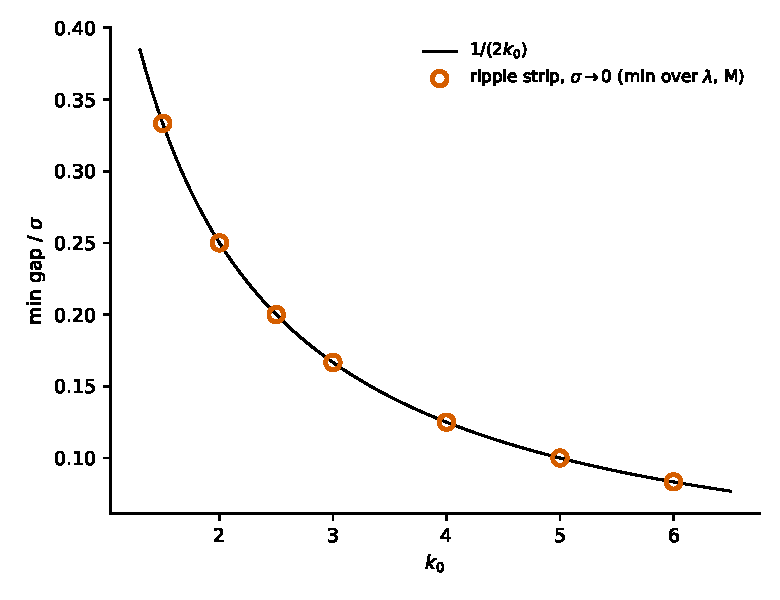
\includegraphics[width=0.85\columnwidth]{figures/fig1_strip_limit.pdf}
\caption{Minimum gap of the strips in the limit $\sigma \to 0$ (computed at $\sigma = 10^{-80}$), at fixed ripple wavenumber $k_0$ and minimised over the other parameters. The line is $1/(2k_0)$.}
\label{fig:strip}
\end{figure}

So the gap in units of $\sigma$ can be made as small as one likes, provided $k_0$ can be made large. The price is the one of Lemma~\ref{lem:smoothing1d}. The blur reduces the ripple's contribution to the sharpness by $e^{-k_0^2}$, so that the window becomes very faint, and the background must become long, $M \gtrsim e^{k_0^2}$, to keep the information along $w$ smaller still. A long background in turn feels the nonlinearity of the pendulum. Balancing these costs at fixed $\sigma$ allows $k_0$ to grow only like $\sqrt{\ln(1/\sigma)}$. At $\sigma = 10^{-80}$, for instance, $k_0 = 7$ is already too expensive: its best gap is $3.28\,\sigma$.

\subsection{The smallest gap at a given resolution}

\begin{observation}
\label{obs:gmin}
The minimum of $g$ over the strips at a given $\sigma$, $g_{\min}(\sigma)$, is listed in Table~\ref{tab:gmin} and shown in Fig.~\ref{fig:gmin}. It decreases to zero. For $\sigma \leq 10^{-24}$ it follows
\begin{equation}
g_{\min}(\sigma) \approx \frac{A}{\sqrt{\ln(1/\sigma) - B}}, \qquad A = 1.02,\quad B = 23.4,
\label{eq:fit}
\end{equation}
with a largest relative residual of $1.1\%$, and the local exponent $d\ln g_{\min}/d\ln\ln(1/\sigma)$ decreases in magnitude from $-1.14$ to $-0.60$ towards $-1/2$. The strips go below the Gaussian-mixture minimum $0.884$ only for $\sigma \lesssim 7.1\times 10^{-6}$.
\end{observation}

\begin{table}[t]
\caption{Smallest gap $g_{\min}(\sigma) = \min (\kappa - R)/\sigma$ over the strips~\eqref{eq:strip}, and the ripple wavenumber $k_0$ of the optimum.}
\label{tab:gmin}
\begin{ruledtabular}
\begin{tabular}{lcc}
$\sigma$ & $g_{\min}$ & $k_0$ \\
\hline
$10^{-2}$ & 1.818 & 0.98 \\
$10^{-4}$ & 1.149 & 1.08 \\
$10^{-5}$ & 0.914 & 1.12 \\
$10^{-6}$ & 0.740 & 1.23 \\
$10^{-12}$ & 0.335 & 1.85 \\
$10^{-24}$ & 0.179 & 3.00 \\
$10^{-48}$ & 0.110 & 4.66 \\
$10^{-96}$ & 0.073 & 6.96 \\
\end{tabular}
\end{ruledtabular}
\end{table}

\begin{figure}[t]
\centering
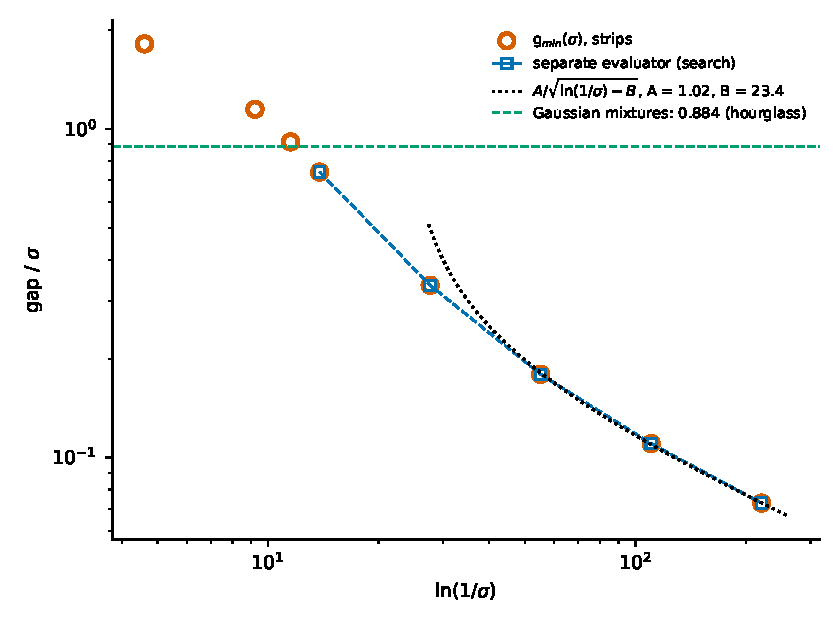
\includegraphics[width=0.9\columnwidth]{figures/fig2_gmin.pdf}
\caption{Smallest gap of the strips at a given $\sigma$ (circles: main evaluators; squares: a separate evaluator used in the search), the fit~\eqref{eq:fit} (dotted), and the minimum over Gaussian mixtures with up to 32 components (dashed).}
\label{fig:gmin}
\end{figure}

The coefficient $A \approx 1$ agrees with the balance above: $g \approx 1/(2k_0)$ with $k_0^2 \approx \ln(1/\sigma)/4$ minus slowly growing corrections. It also agrees with the proved side. On the strip optima $\xb(\sqrt\varrho)$ approaches $k_0^2$ as $\sigma\to 0$ (at $\sigma = 10^{-96}$, $\xb(\varrho) = 48.2$ and $K_\Lambda = 0.99$, against $k_0^2 = 48.4$), so that Corollary~\ref{cor:regular} gives $g \gtrsim 1/(\pi\sqrt2\,k_0)$. This is below the observed $1/(2k_0)$ by the factor $\pi/\sqrt2 \approx 2.2$ lost in Eq.~\eqref{eq:PwP}, the dominant looseness of Theorem~\ref{thm:log} on the strips.

We also searched beyond the single strip, at $\sigma = 10^{-12}$ and $10^{-24}$: superpositions of the wavenumbers $k$ and $2k$, three interfering windows with free phases, windows with different $k_0$ side by side along $w$, and the first three harmonics. None went below the single strip; the best members were higher by $0.07\%$ to $1.6\%$, and the optimiser removed the extra components. This agrees with Lemma~\ref{lem:smoothing1d}, in which equality requires a single wavenumber, but the search was local.

\subsection{How the numbers were checked}

The gap of the strips is a small difference of large quantities. At $\sigma = 10^{-24}$, for instance, the numerator of Eq.~\eqref{eq:formula} is of order $10^{-34}$ while its building blocks are many orders of magnitude larger, and a direct evaluation fails; an early version of this study was misled by a rounding artefact in one of the building blocks (Appendix~\ref{app:methods}). Every value in Table~\ref{tab:gmin} was therefore computed by at least two evaluators that share no code for the states, the pointwise fields or the integration, including a full two-dimensional grid where feasible and a 320-digit pointwise check. In addition, the values at $\sigma = 10^{-4}$, $10^{-6}$, $10^{-12}$, $10^{-24}$ and $10^{-48}$ were reproduced to ten digits or better by an evaluator written separately from the closed-form expressions of Appendix~\ref{app:methods}, whose formulas were in turn checked pointwise against direct two-dimensional quadrature of the posterior; an optimisation with that evaluator from unrelated starting points found the same optima at $\sigma = 10^{-12}$ and $10^{-24}$.
